\chapter{Introduksjon}


\section{Om applikasjonen}
\begin{itemize}
\item All kode i applikasjonen er på engelsk med hensikt til at denne skal eventuelt kompileres på forskjellige miljøer med ulike typer \"encoding\". 
\item Kompilert med SDK versjon 23: Android 6.0 Marchmallow, Build tools: 23.0.0
\item Mål SDK: API 21: Android 5.0 (Lollipop) Minimal SDK: API 19: Android 4.4 (KitKat)
\item ID for applikasjonen: com.example.s198569.hangman
\item Utviklingsmiljø: Android Tools 1.3.2, Fedora Linux 22 x64
\item Debugging og testing gjennomført på LGE Optimus 2X (P990) med Cyanogenmod Android 4.4.4. Enheten har samme skjermstørrelse som målenhet Samsung Nexus S.
\end{itemize}


\section{Hva er implementert og hva har jeg lært meg?}
Jeg har aldri før utviklet for Android derfor er alle komponenter som jeg bruker i applikasjonen nye for meg. Jeg hatt som mål å strekke meg noe utøver de krav som er beskrevet i oppgavebeskrivelsen. Følgende liste er et sammendrag over de komponenter som er implementert i applikasjonen utøver de som vært introdusert i forelesningene:

\begin{description}

\item[SQLite] Lagring og lesing av data i appens interne \texttt{SQLite} database.

\item[Styles] Egne stiler for flere komponenter. Eksempel på dette er egne stiler som er brukt i f.eks. \texttt{GamePlayActivity} der det er opprettet egne stiler både for knapper og \texttt{EditText} som benyttes til å vise ord som skal gjettes.

\item[Native preferances] Bruk av \texttt{PreferanceActivity} for å vise innstillinger for applikasjonen på en oversiktlig og ryddig måte. 

\item[Dynamiske komponenter] Opprette grafiske komponenter på en dynamisk måte. Eksempel på dette er tastatur som blir satt opp avhengig av det språk som er valgt for systemet eller applikasjonen (tastaturet blir satt opp fra et predefinert xml fil som inneholder alle bokstaver fra det språket). Alt dette skjer i samme aktivitet, det brukes ingen hardkoding av aktiviteter.

\item[Endring av språk fra app] Endre språk i applikasjonen uten at språk for systemet blitt endret. Det valgte språket blir også bevart dersom applikasjonen roteres. 

\item[Animasjoner] På hovedaktiviteten vises det en animasjon av en «Hangman» som er opprettet manuelt i xml resurser (se \texttt{res $\rightarrow$ anim}). Det er også brukt xml animasjoner på logo slik at den blir vist sakte fra gjennomsiktig bakgrunn (\textit{fade}).

\end{description}



\chapter{Bruksanvisning og aktiviteter}
I følgende kapittel beskrives det hvordan det er tenkt at spillet skal brukes samt en enkel navigasjon mellom applikasjonens skjermbilder. 

\section{Oppstart av applikasjonen}
Når applikasjonen startes blir brukeren presentert av skjermbilde presentert i figur \ref{fig:activity_front}. 
\begin{figure}[ht]
\centering
 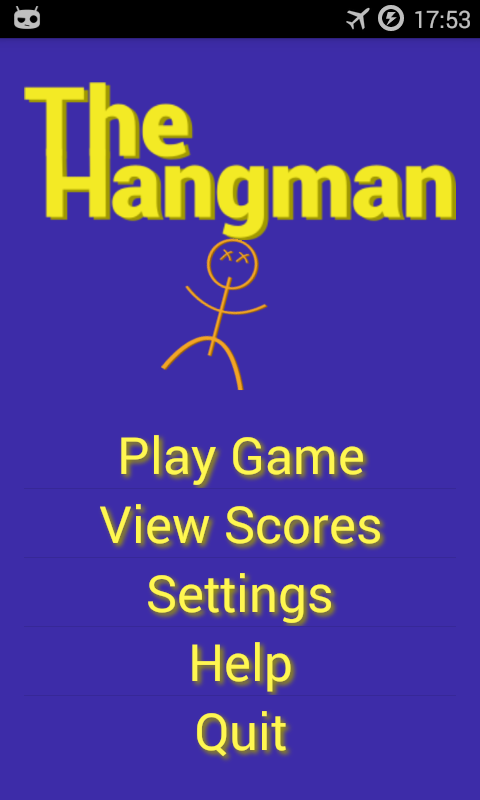
\includegraphics[scale=0.25]{./img/bruksanvisning/1.png}
 \caption{Startskjerm for Hangman}
 \label{fig:activity_front}
\end{figure}

Fra dette bilde er det mulig for spilleren å: 
\begin{description}
\item[Play Game] Starte nytt spill. Dette vil ta spilleren til neste skjermbilde der det er mulig å registrere en ny spiller eller velge allerede eksisterende spillere som er registrert fra før.
\item[View Scores] Se på en sammenstilling av poeng for registrerte spillere. Sammenstillingen er sortert etter total poengsum synkende.
\item[Settings] Innstillinger for appen som valg av språk og lyd på eller av (lydeffekter er ikke implementert ennå).
\item[Help] Skjermbilde med regler for applikasjonen informasjon om applikasjonen. 
\item[Quit] Avlutter applikasjonen. 
\end{description}


\section{Nytt spill}

Spilleren blir presentert med et skjermbilde for å starte nytt spill , figur \ref{fig:registrering}. Her er det mulig å starte et nytt spill gjennom å registrere en ny spiller eller fortsette som en spiller som allerede er registrert fra før. Figur \ref{fig:ny_spiller} viser tilnærming for registrering av en ny spiller. Her blir brukeren varslet om at et nytt brukernavn er registrert via en \texttt{toast} og spurt dersom man ønsker å fortsette å spille med den nye spilleren. Spillet starter og et nytt brukernavn er presenter på spille aktiviteten i nord-vestre hjørne , figur \ref{fig:spill_igang}.

\begin{figure}[ht]
    \centering
    \begin{subfigure}[b]{0.3\textwidth}
        
\includegraphics[width=\textwidth]{./img/bruksanvisning/2.png}
        \caption{Registrering}
        \label{fig:registrering}
    \end{subfigure}
    \begin{subfigure}[b]{0.3\textwidth}
        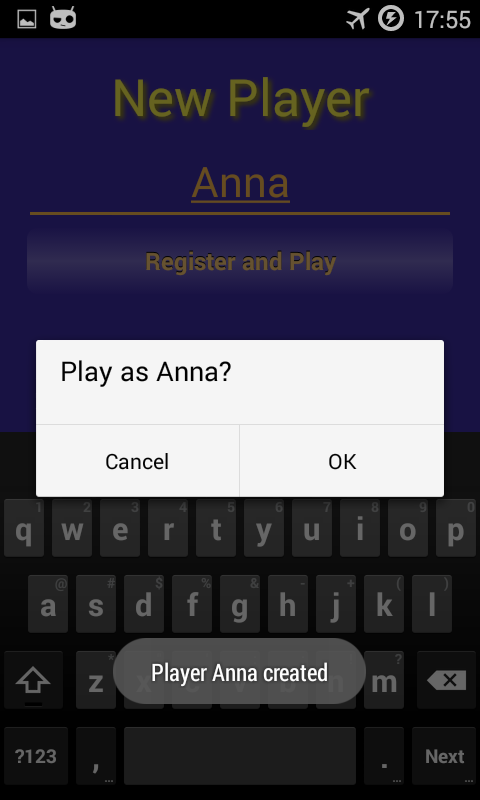
\includegraphics[width=\textwidth]{./img/bruksanvisning/3.png}
        \caption{Ny spiller registrert}
        \label{fig:ny_spiller}
    \end{subfigure}
    \begin{subfigure}[b]{0.3\textwidth}
        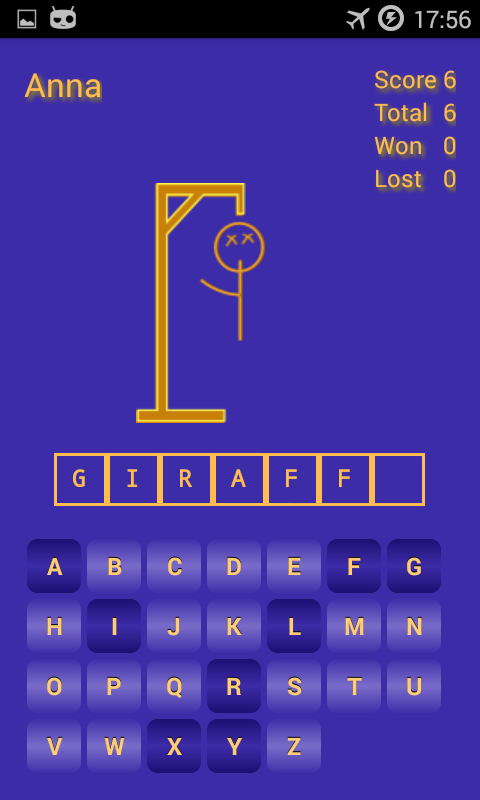
\includegraphics[width=\textwidth]{./img/bruksanvisning/4.png}
        \caption{Pågående spill}
        \label{fig:spill_igang}
    \end{subfigure}
    \caption{Nytt spill med en ny spiller}\label{fig:new_game_activities}
\end{figure}

Etter et spilleren har gjettet alle ord og vunnet eller ha misslykket med å avsløre hvilket ord som skjler seg bak firkantene blir spilleren spurt om man ønsker å spille én gang til, figur \ref{fig:fortsette}. Dersom det svares ja startes et nytt spill i samme økt. Dersom man har spilt minst et spill i økten blir spilleren presentert med enkel statistikk for den pågående økten i nord-østlig hjørne, se figur \ref{fig:nyt_spill_samme_okt}. I statistikken presenteres: (1) aktuelt antall poeng, (2) totalt antall poeng som spilleren har tjent sammen i pågående økt, (3) antall spill som er vunnet i økten samt (4) antall spill som er tapt. 

\begin{figure}[ht]
    \centering
    \begin{subfigure}[b]{0.3\textwidth}
        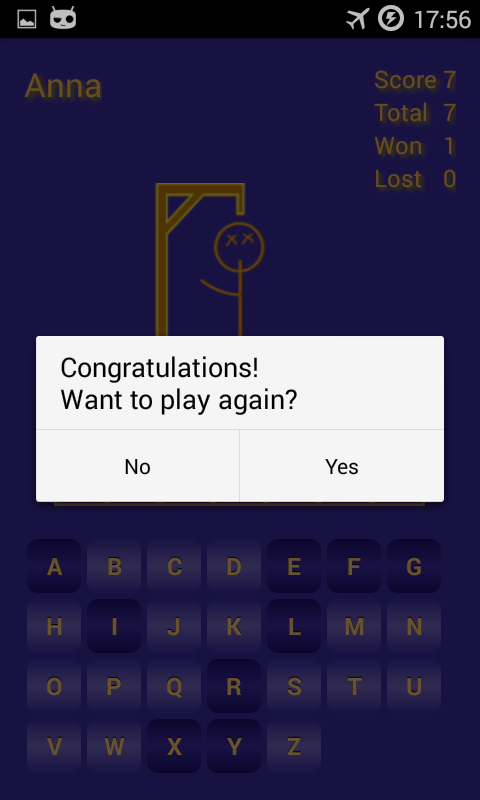
\includegraphics[width=\textwidth]{./img/bruksanvisning/5.png}
        \caption{Fortsette?}
        \label{fig:fortsette}
    \end{subfigure}
    \begin{subfigure}[b]{0.3\textwidth}
        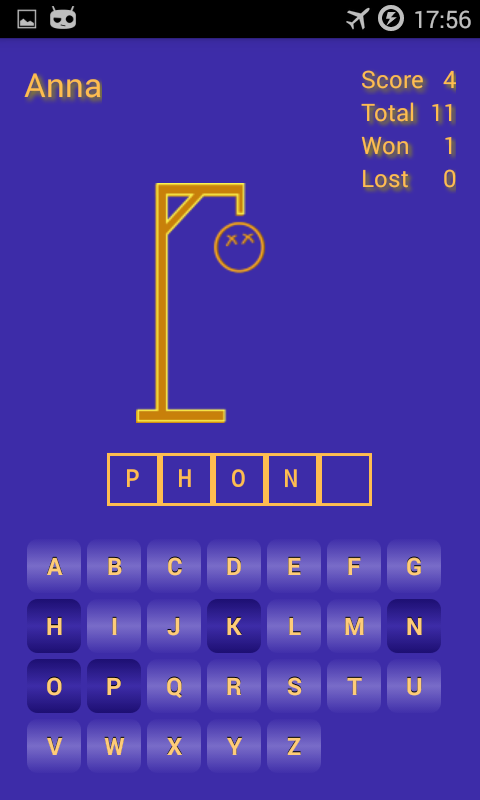
\includegraphics[width=\textwidth]{./img/bruksanvisning/6.png}
        \caption{Nytt spill}
        \label{fig:nyt_spill_samme_okt}
    \end{subfigure}
    \caption{Nytt spill i samme økt}\label{fig:new_game_activities}
\end{figure}


\section{Innstillinger}
I oppgaven skal det implementeres mulighet til endring av språk i applikasjonen uten en endring av systeminnstillinger. For å implementere slik funksjonalitet er det brukt \texttt{PreferenceActivity} som tillater en ryddig oppsamling av alle innstillinger som skal brukes i applikasjonen. Aktivitet med innstillinger startes har hoved menyen med \texttt{Settings} hvilken deretter starter aktivitet som presenteres i figur \ref{fig:innstllinger_oversikt}. Her blir det presentert en liste med alle mulige innstillinger i applikasjonen (anm. innstilling av skru på og av lyd er foreløpig ikke implementert ettersom det er ingen lydeffekter som er implementert i den versjonen). Brukeren har dog mulighet å endre språk for hele applikasjonen og blir presentert med en liste av alle aktuelt tilgjengelige språk, figur \ref{fig:innstllinger_velg_sprak}. Dersom brukeren velger et annet språk enn hva som er aktivt blir det presentert en kort advarsel om at dette er en \textit{alpha} funksjonalitet, figur \ref{fig:innstillinger_advarsel}. Jeg har valgt å varsle brukeren om dette ettersom det er en ikke anbefalt måte å endre språk på i en kjørende applikasjon. Det er noe som skal helt gjøres fra systemets språkinnstillinger ettersom Android systemet er satt opp på en måte som forsøker starte alle nye aktiviteter i det språk som er aktivt i systemet. Dette danner noen utfordringer under blant annet rotasjon av skjermen da det må lages spesiell kode i hver aktivitet som tar høyde for at applikasjonen kommer til å forsøke å overgå til standardspråk etter at orienteringen er endret.


\begin{figure}[ht]
    \centering
    \begin{subfigure}[b]{0.3\textwidth}
        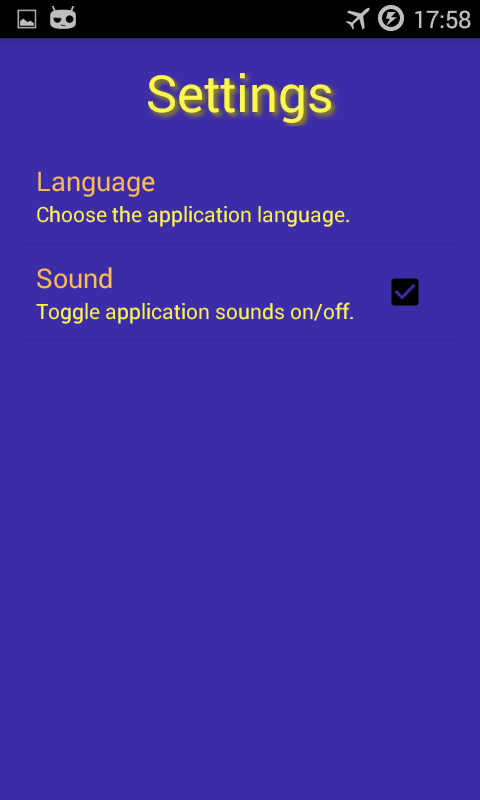
\includegraphics[width=\textwidth]{./img/bruksanvisning/7.png}
        \caption{Oversikt}
        \label{fig:innstllinger_oversikt}
    \end{subfigure}
    \begin{subfigure}[b]{0.3\textwidth}
        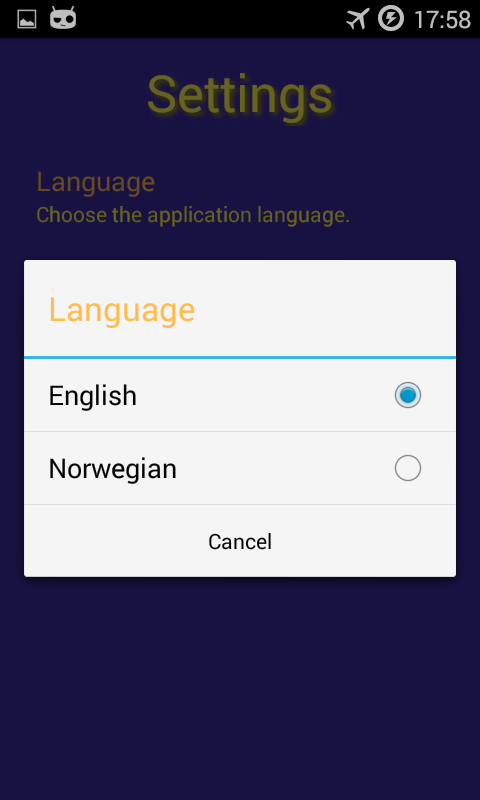
\includegraphics[width=\textwidth]{./img/bruksanvisning/8.png}
        \caption{Valg av språk}
        \label{fig:innstllinger_velg_sprak}
    \end{subfigure}
    \begin{subfigure}[b]{0.3\textwidth}
        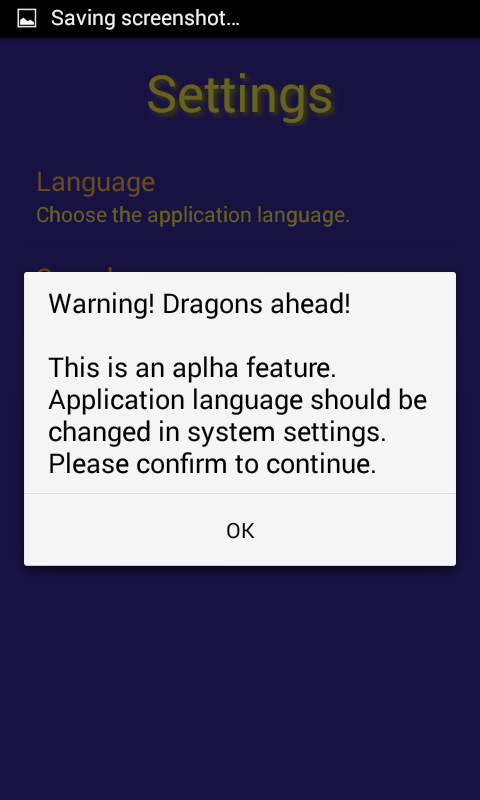
\includegraphics[width=\textwidth]{./img/bruksanvisning/9.png}
        \caption{Advarsel}
        \label{fig:innstillinger_advarsel}
    \end{subfigure}
    \caption{Innstillinger}\label{fig:innstillinger}
\end{figure}

Etter at språk blir endret blir aktiviteten med innstillinger lukket og fokus flyttes automatisk til hovedaktiviteten der alle grafiske komponenter blir opprettet på nytt med et nytt språk. Språkendringen gjelder også spillaktivitet der det dynamisk blir opprettet nytt tastatur med spesifikke tegn for språket (dersom nødvendig) og ordlisten i spillet blir skiftet ut slik at spillet kan tas på det språk som brukeren har valgt, figur \ref{fig:spill_norsk}. Konfigurasjon for tastatur er lagret i \texttt{res $\rightarrow$ values $\rightarrow$ alphabet.xml}.

\begin{figure}[ht]
    \centering
   \begin{subfigure}[b]{0.3\textwidth}
        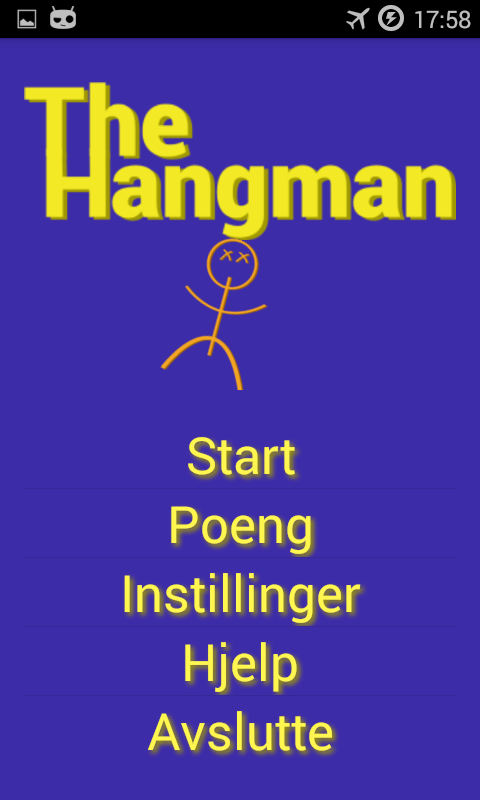
\includegraphics[width=\textwidth]{./img/bruksanvisning/10.png}
        \caption{Språk endret}
        \label{fig:innstillinger_endret}
    \end{subfigure}
    \begin{subfigure}[b]{0.3\textwidth}
        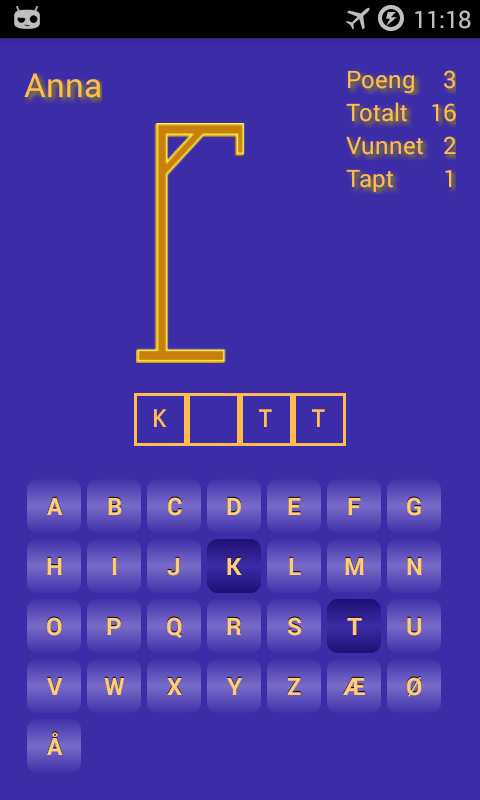
\includegraphics[width=\textwidth]{./img/bruksanvisning/11.png}
        \caption{Nytt språk i spillet}
        \label{fig:spill_norsk}
    \end{subfigure}
    \caption{Språkinnstillinger endret}\label{fig:innstillinger_endret_norsk}
\end{figure}



\section{Øvrige aktiviteter}
De øvrige aktiviteter som er implementert er (1) aktivitet for oversikt over poeng sammenstilling for alle registrerte spillere og (2) en aktivitet som viser hjelp og regler for spillet. Aktivitet for «High Score» viser alle registrerte spillere og sorterer resultat synkende fra de brukere som har høgste score i spillet, figur \ref{fig:aktivitet_score}. Aktivitet for «Hjelp» er satt opp av vanlig \texttt{TextView} og i tillegg tekst som vises blir formatert med hjelp av html tagger, figur \ref{fig:aktivitet_hjelp}. Begge aktivitetene blir endret hvis brukeren bytter språk i applikasjonen eller i systemet. 

\begin{figure}[ht]
    \centering
   \begin{subfigure}[b]{0.3\textwidth}
        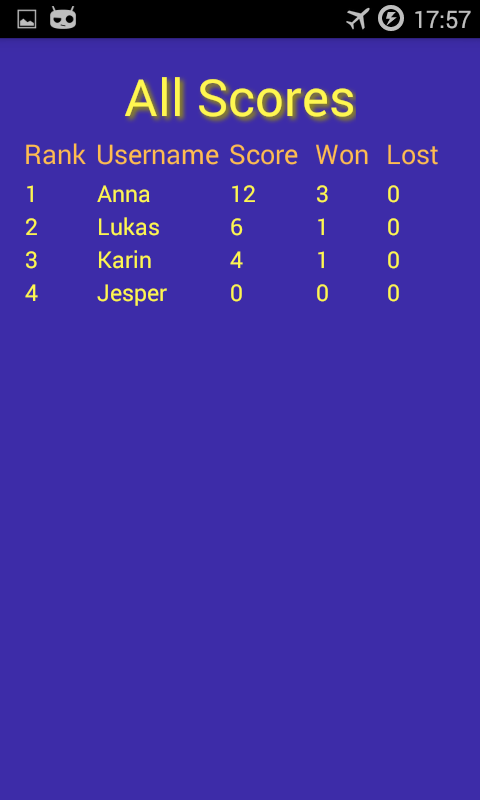
\includegraphics[width=\textwidth]{./img/bruksanvisning/12.png}
        \caption{High score}
        \label{fig:aktivitet_score}
    \end{subfigure}
    \begin{subfigure}[b]{0.3\textwidth}
        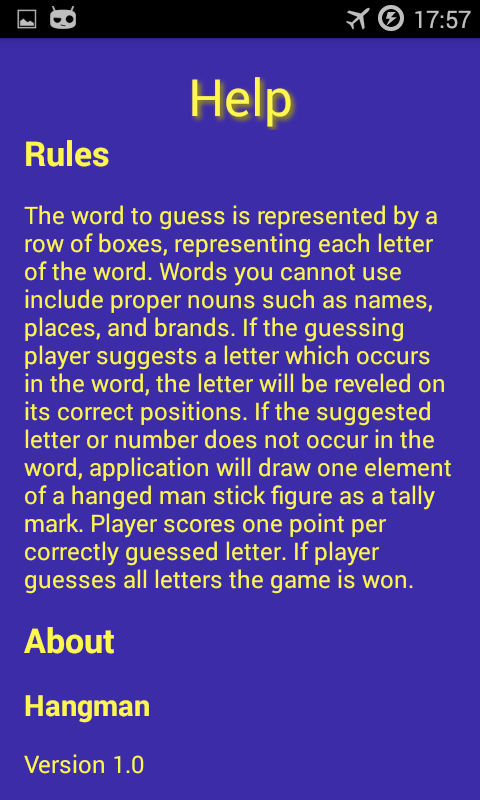
\includegraphics[width=\textwidth]{./img/bruksanvisning/13.png}
        \caption{Hjelp}
        \label{fig:aktivitet_hjelp}
    \end{subfigure}
    \caption{Øvrige aktiviteter}\label{fig:aktiviteter_ovrige}
\end{figure}



\chapter{Klasser og struktur}

\begin{description}
\item[\underline{\texttt{StartGameActivity}}] Klasse som har ansvar for å starte hovedaktiviteten i applikasjonen. 

\begin{description}

\item[\texttt{LoginActivity}]
Denne klassen sørger for å opprette nye brukere eller å logge på eksisterende brukeres som allerede er registrert i spiller. Klassen har en leseforbindelse med databasen. 

\item[\texttt{GamePlayActivity}]
Dette er den største klassen i applikasjonen. Klassen sørger for å opprette en ny økt med spill og kjøre kontinuerlige spillomganger frem til brukeren velger å avslutte eller at ordene tar slutt.

\item[\texttt{HangmanPreferencesActivity}]
Klassen brukes til å starte aktiviteten til innstillinger for programmet. Klassen inneholder klikklytter til listen av innstillinger samt trigger eventuelle dialoger for å skifte språk som vises til brukeren. Dersom språk blir endret lagres det en flagg i \texttt{SharedPreferences} og hoved aktiviteten startes på nytt. 

\item[\texttt{ScoresActivity}]
Klassen har som oppgave å gjøre en forespørsel til DAO klassen\footnote{\texttt{HangmanDataSource}} med hensikt å hente inn en liste over eksisterende brukere og sortere de synkende etter totalt antall opptjente poeng (\textit{leaderboard}).

\item[\texttt{HelpActivity}]
Klassen viser en statisk tekst over spileregler og noen informasjon om applikasjonen. Teksten hentes fra \texttt{strings.xml} og blir internt formatert med html tagger. 

\end{description}

\item[\underline{\texttt{lib}}] 
Pakke med hjelpeklasser. Her er det samlet alle klasser som brukes i form av hjelpeklasser for applikasjonen. 
\begin{description}

\item[\texttt{HangmanDatabase}]
Klassen instanser \texttt{SQLite} database gjennom å arve klassen \texttt{SQLiteOpenHelper}. Klassen brukes til å opprette tabellen i databasen samt har \textit{override} for alle nødvendige metoder som kreves av klassen som arves.

\item[\texttt{HangmanDataSource}]
Dette er hjelpklassen som instanserer \texttt{HangmanDatabase} og implementerer alle nødvendige metoder som brukes til lesing, skriving og henting og behandling av den data som blir hentet fra databasen. Eksempel på dette er oppdatering av spiller score, henting av alle spillere på tabellform og diverse data om spillerne.

\item[\texttt{WordsProvider}]
Klassen brukes til å hente alle tilgjengelige ord til det språk som er valgt i applikasjonen. Klassen benytter seg av \texttt{Collections} klassen i Java slik at alle ord blir lastet inn fra \texttt{res $\rightarrow$ values $\rightarrow$ arrays.xml}. Klassen bruker internt en \texttt{ArrayList} i hvilken alle ord fra filen blir plasser. Listen blir randomisert for hver ny økt med hjelp av \texttt{Collections.shuffle()} slik at rekkefølgen blir alltid forskjellig. 


\item[\texttt{Player}]
Klassen representerer en abstraksjon av spiller i spillet som brukes for å midlertidig lagre alle nødvendige data om spilleren. \texttt{Player} objekt blir opprettet hver gang det registreres ny spiller eller hentes inn en eksisterende fra databasen. Spiller objektene tas vare på så lenge spilleøkte varer, så snart det avsluttes at spill i samme økt. For hvert nytt spill blir spillerens rad oppdatert i databasen med nye poeng som brukeren har tjent opp i spillet.

\end{description}


\end{description}


\begin{landscape}
\begin{figure}[ht]
\centering
 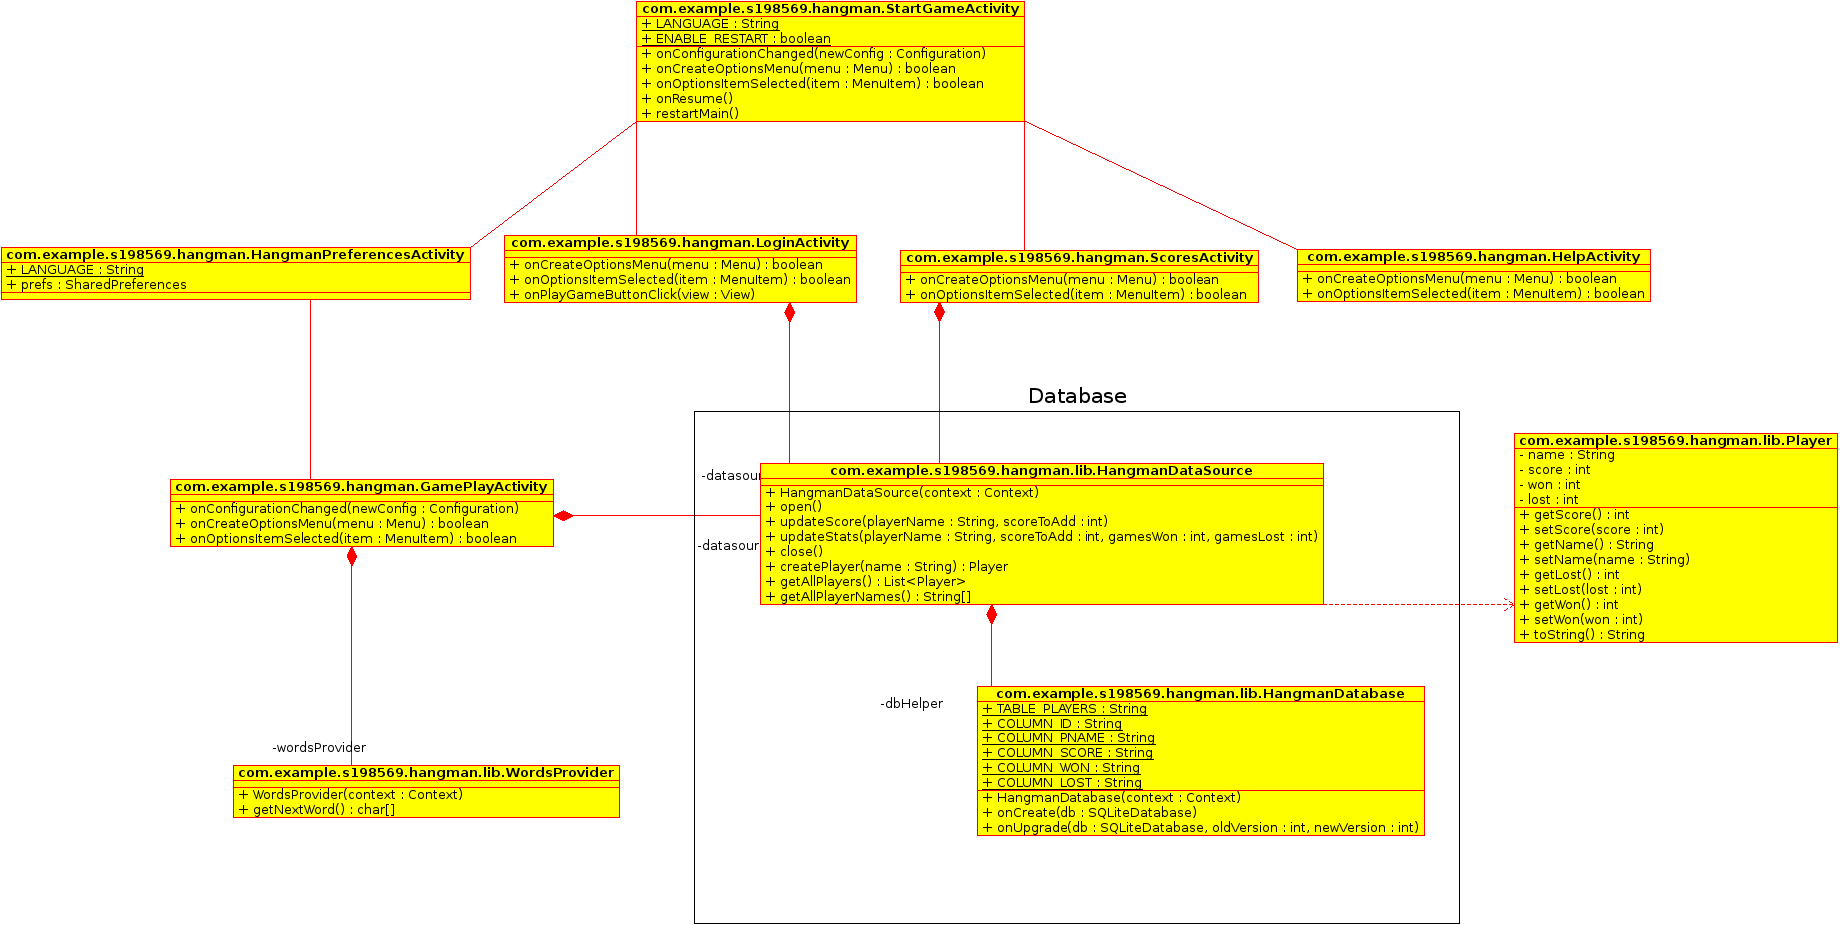
\includegraphics[width=\hsize]{./uml/classdiagram.png}
 \caption{Klassediagram}
 \label{fig:klassediagram}
\end{figure}

\end{landscape}



\chapter{Presentasjon av løsninger}

\textbf{\emph{I følgende avsnitt presenteres det kodeeksempel over de viktigste løsninger fra applikasjonens klasser. For innføring i resterende klasser i metoder henvises det til den innleverte kildekoden.}}

\section{Lagring av data}

\subsection{\texttt{HangmanDatabase.java}}
Applikasjonen benytter seg av en SQLite database for å ta vare på navn til spillere og total opptjent poengsum for hver enkel spiller. Det lagres også totalt antall spill som hver bruker har vunnet og tapt. Hvordan tabellen i databasen blir dannet presenteres i kodeeksempel \ref{code:tabell_opp}.

\begin{lstlisting}[language=Java, caption=Script for opprettelse av tabell, label=code:tabell_opp]
 private static final String DATABASE_CREATE =
            "create table " + TABLE_PLAYERS + "(" +
                    COLUMN_ID + " integer primary key autoincrement, " +
                    COLUMN_PNAME + " text not null, " +
                    COLUMN_SCORE + " integer, " +
                    COLUMN_WON + " integer, " +
                    COLUMN_LOST + " integer" +
                    ");";
\end{lstlisting}


\subsection{\texttt{HangmanDataSource.java}}
Klassen inneholder en hjelpemetode \texttt{cursorToPlayer} som tar in parameter cursor og henter inn datafelt som plasseres i spilleobjektet. Kodeeksempel \ref{code:cursor_help}

\begin{lstlisting}[language=Java, caption=Hjelpemetode for plasering av cursor, label=code:cursor_help]
private Player cursorToPlayer(Cursor cursor){
        Player player = new Player();
        player.setName(cursor.getString(1));
        player.setScore(cursor.getInt(2));
        player.setWon(cursor.getInt(3));
        player.setLost(cursor.getInt(4));
        return player;
    }
\end{lstlisting}

I kodeeksempel \ref{code:tabell_ny_spiller} presenteres det kode som sørger for å opprettelse av en ny spiller i tabellen. Etter innsetting i tabellen benyttes det \texttt{insertId} variabel som blir returnert fra insert metoden til databasen. Denne id benyttes deretter for å finne frem til riktig spiller i tabellen, det vil si at den spiller som blir dannet der blir også returnert fra databasen og med hjelp av eksempel \ref{code:cursor_help} blir det dannet et spiller objekt som returneres tilbake. Slik tilnærmingsmåte sørger for at spilleren blir lagt inn i databasen ettersom det benyttes felt som er lagret i databasen og ikke de felt som allerede eksisterer i det aktive objektet.

\begin{lstlisting}[language=Java, caption=Metode for oppretting av en ny spiller i tabellen, label=code:tabell_ny_spiller]
public Player createPlayer(String name){
        ContentValues values = new ContentValues();
        values.put(HangmanDatabase.COLUMN_PNAME, name);
        values.put(HangmanDatabase.COLUMN_SCORE, 0);
        values.put(HangmanDatabase.COLUMN_WON, 0);
        values.put(HangmanDatabase.COLUMN_LOST, 0);

        long insertId = database.insert(HangmanDatabase.TABLE_PLAYERS, null, values);

        if(insertId < 0){
            Log.d("HANGMAN", "Could not insert into table.");
        }else{
            Log.d("HANGMAN", "Insertion into table successful");
        }

        Cursor cursor = database.query(HangmanDatabase.TABLE_PLAYERS,
                allColumns, HangmanDatabase.COLUMN_ID + " = " + insertId, null,
                null, null, null);

        cursor.moveToFirst();
        Player newPlayer = cursorToPlayer(cursor);
        cursor.close();

        return newPlayer;
    }
\end{lstlisting}

For å hente \textit{High Score} liste benyttes det kode som er presentert i kodeeksempel \ref{code:tabell_alle_spillere}. I presentert eksempel blir spillere hentet inn til peker og sortert direkte i pekeren etter poengkolonnen. Så lenge det eksisterer data som kan plasseres i pekeren opprettes det nye spiller objekter fra data som finnes i databasen og til slutt returneres det en sortert listen med spiller objekter.

\begin{lstlisting}[language=Java, caption=Innheting av alle spiller og sortering, label=code:tabell_alle_spillere]
public List<Player> getAllPlayers(){
        List<Player> players = new ArrayList<Player>();

        Cursor cursor = database.query(HangmanDatabase.TABLE_PLAYERS, allColumns, null, null, null, null, HangmanDatabase.COLUMN_SCORE + " DESC");
        if(cursor == null ) return null;
        cursor.moveToFirst();

        while(!cursor.isAfterLast()){
            Player player = cursorToPlayer(cursor);
            players.add(player);
            cursor.moveToNext();
        }

        cursor.close();
        return players;
    }
\end{lstlisting}


\section{Internasjonalisering}
I klassen \texttt{HangmanPreferencesActivity.java} blir det endret språk utefra valg til brukeren. Dette blir gjennomført gjennom å oppdatere lokale innstillinger til applikasjonen samt lagret i \texttt{SharedPreferences} hvilket språk som skal benyttes, kodeeksempel \ref{code:bytte_sprak}. Deretter startes hovedaktivitet på nytt for å ta i bruk endringer. Ettersom det blir lagret i felles innstillinger hvilket språk som skal benyttes i applikasjonen er den verdien tilgjengelig for alle aktiviteter. Derfor etter bytte av orientering av skjermen vil applikasjonen blir startet om og systemet kommer til å forsøke å sette samme språk på applikasjonen som det er definiert på systemet. 

\begin{lstlisting}[language=Java, caption=Metode for språkbytte, label=code:bytte_sprak]
    private void changeLanguage(String locale_language) {
        Locale locale = new Locale(locale_language);
        Locale.setDefault(locale);
        Configuration config = new Configuration();
        config.locale = locale;
        getApplicationContext().getResources().updateConfiguration(config, null);

        //Saving the chosen language to open it up inside the main activity
        SharedPreferences.Editor spEdit = prefs.edit();
        spEdit.putString(LANGUAGE, locale_language);
        spEdit.apply();

        //Starting main activity
        StartGameActivity.ENABLE_RESTART = true;
        Intent i = new Intent(this, StartGameActivity.class);
        i.addFlags(Intent.FLAG_ACTIVITY_CLEAR_TOP | Intent.FLAG_ACTIVITY_SINGLE_TOP);
        startActivity(i);
    }
\end{lstlisting}

Dette forebygges gjennom at kontrollere den verdi som er lagret i felles innstillinger med dem som applikasjonen kjører etter rotasjon av skjerm gjennom:
\begin{lstlisting}[language=Java]
getResources().getConfiguration().locale.getDisplayLanguage() 
\end{lstlisting}
Dersom den lagrede veriden overensstemmer ikke med den aktuelle verdien for språket fremtvinges en omstart av aktiviteten med nytt språk med hjelp av kode i eksempel \ref{code:bytte_sprak_rotasjon}.

\begin{lstlisting}[language=Java, caption=Språkkontroll etter rotasjon, label=code:bytte_sprak_rotasjon]
    public void onConfigurationChanged(Configuration newConfig) {
        super.onConfigurationChanged(newConfig);
        setContentView(R.layout.activity_start_game);

        initilizeGuiComponents();

        Log.w("HANGMAN", "appLocale "+appLocale);
        String currentLocale = getResources().getConfiguration().locale.getDisplayLanguage();
        Log.w("HANGMAN", "currentLocale "+currentLocale);

        if(!appLocale.equals(currentLocale)){
            switch (appLocale){
                case "norsk bokmal":
                    changeLanguage("nb_NO");
                    break;
                case "English":
                    changeLanguage("en_US");
                    break;
                default:
                    changeLanguage("en_US");
                    break;
            }
        }
    }
\end{lstlisting}


Etter at språk er endret endres også alle dynamiske komponenter som f.eks. tastatur som blir opprettet fra lokalisert xml fil hvilken hentes fra \texttt{values/alphabet.xml} samt \texttt{values-nb/alphabet.xml}. Denne filen ligger til grunn den endring som foretas i tastaturet som presenteres i figur \ref{fig:aktiviteter_spill_internasjonalisering}.

\begin{figure}[ht]
    \centering
   \begin{subfigure}[b]{0.3\textwidth}
        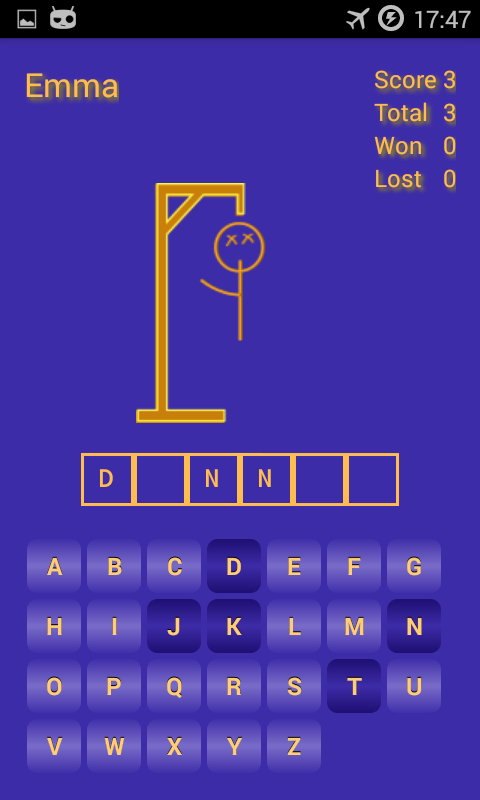
\includegraphics[width=\textwidth]{./img/losninger/1.png}
        \caption{Engelsk versjon}
        \label{fig:aktivitet_engelsk}
    \end{subfigure}
    \begin{subfigure}[b]{0.3\textwidth}
        
\includegraphics[width=\textwidth]{./img/losninger/2.png}
        \caption{Norsk versjon}
        \label{fig:aktivitet_norsk}
    \end{subfigure}
    \caption{Internasjonalisering av spillaktivitet}
    \label{fig:aktiviteter_spill_internasjonalisering}
\end{figure}



\section{Grafiske komponenter}
De brukes noen komponenter som er opprettet gjennom en egen. 



\chapter{Utfordringer}
\section{Rotasjon}
Her skal man forklare forskjellen mellom å lagre status av skjermen på den gamle måten og den nye i systemet. Hvordan de forskjellige komponentene lastes om. 
\begin{lstlisting}[language=Java]
    @Override
    protected void onSaveInstanceState(Bundle outState) {
        super.onSaveInstanceState(outState);

        outState.putString(PLAYERNAME, pName);
        outState.putInt(LETTERSCOUNT, lettersCount);
        outState.putCharArray(LETTERS, letters);
        outState.putInt(GAMESCORE, gameScore);
        outState.putInt(SESSIONSCORE, sessionScore);
        outState.putInt(TRYCOUNT, tryCount);
        outState.putInt(LETTERSGUESSED, lettersGuessed);
        outState.putInt(GAMESWON, gamesWon);
        outState.putInt(GAMESLOST, gamesLost);

        Toast.makeText(this, "Data er lagret", Toast.LENGTH_SHORT).show();

    }
\end{lstlisting}

\begin{lstlisting}
 @Override
    protected void onRestoreInstanceState(Bundle savedInstanceState) {
        super.onRestoreInstanceState(savedInstanceState);


        pName = savedInstanceState.getString(PLAYERNAME);
        lettersCount = savedInstanceState.getInt(LETTERSCOUNT);
        letters = savedInstanceState.getCharArray(LETTERS);
        gameScore = savedInstanceState.getInt(GAMESCORE);
        sessionScore = savedInstanceState.getInt(SESSIONSCORE);
        tryCount = savedInstanceState.getInt(TRYCOUNT);
        lettersGuessed = savedInstanceState.getInt(LETTERSGUESSED);
        gamesWon = savedInstanceState.getInt(GAMESWON);
        gamesLost = savedInstanceState.getInt(GAMESLOST);

        updateHangmanImage();
        Toast.makeText(this, "Restoring game score: "+gameScore, Toast.LENGTH_SHORT).show();

        playerName.setText(pName);
        gameScoreView.setText(String.valueOf(gameScore));
        sessionScoreView.setText(String.valueOf(sessionScore));
        gameScoreView.setText(String.valueOf(gamesWon));
        sessionScoreView.setText(String.valueOf(sessionScore));
    }
\end{lstlisting}


